\section{Pre-Commissioning and Installation}

In this section we describe the procedures that took
place after chamber stringing was complete in order to get the
chambers ready for installation and to install them 
in Hall~B.

\subsection{Electronics Installation and Turn-on}
\label{electronics-installation}

After the chambers were strung and went through a mechanical quality
check to insure that all wires were intact and properly tensioned, we
installed the on-chamber electronics boards, using
the following procedures:
\begin{enumerate}
\item ``daisy-chained'' the field wire crimp pins so that a single
high voltage cable could power two rows of field wires (32 wires);
\item physically positioned the boards so that their plated-through
holes aligned directly above the sense wire crimp pins, and attached
the boards to the chamber with screws;
\item electrically connected each sense wire crimp pin to each
plated-through hole using a conductive elastomer tube that fit
over the crimp pin and also contacted the plated-through hole on
its outer radius.
\end{enumerate}
A sketch of the process of attaching the circuit boards to the 
chambers is shown in Fig.~\ref{mounting-stb}.

%%%%%%%%%%%%%%%%%%%%%%%%%%%%%%%%%%%%%%%%%%%%%%%%%%%%%%%%%%%%%
\begin{figure}[htbp]
\vspace{2.7cm}
\begin{picture}(50,50)
\put(13,-5)
{\hbox{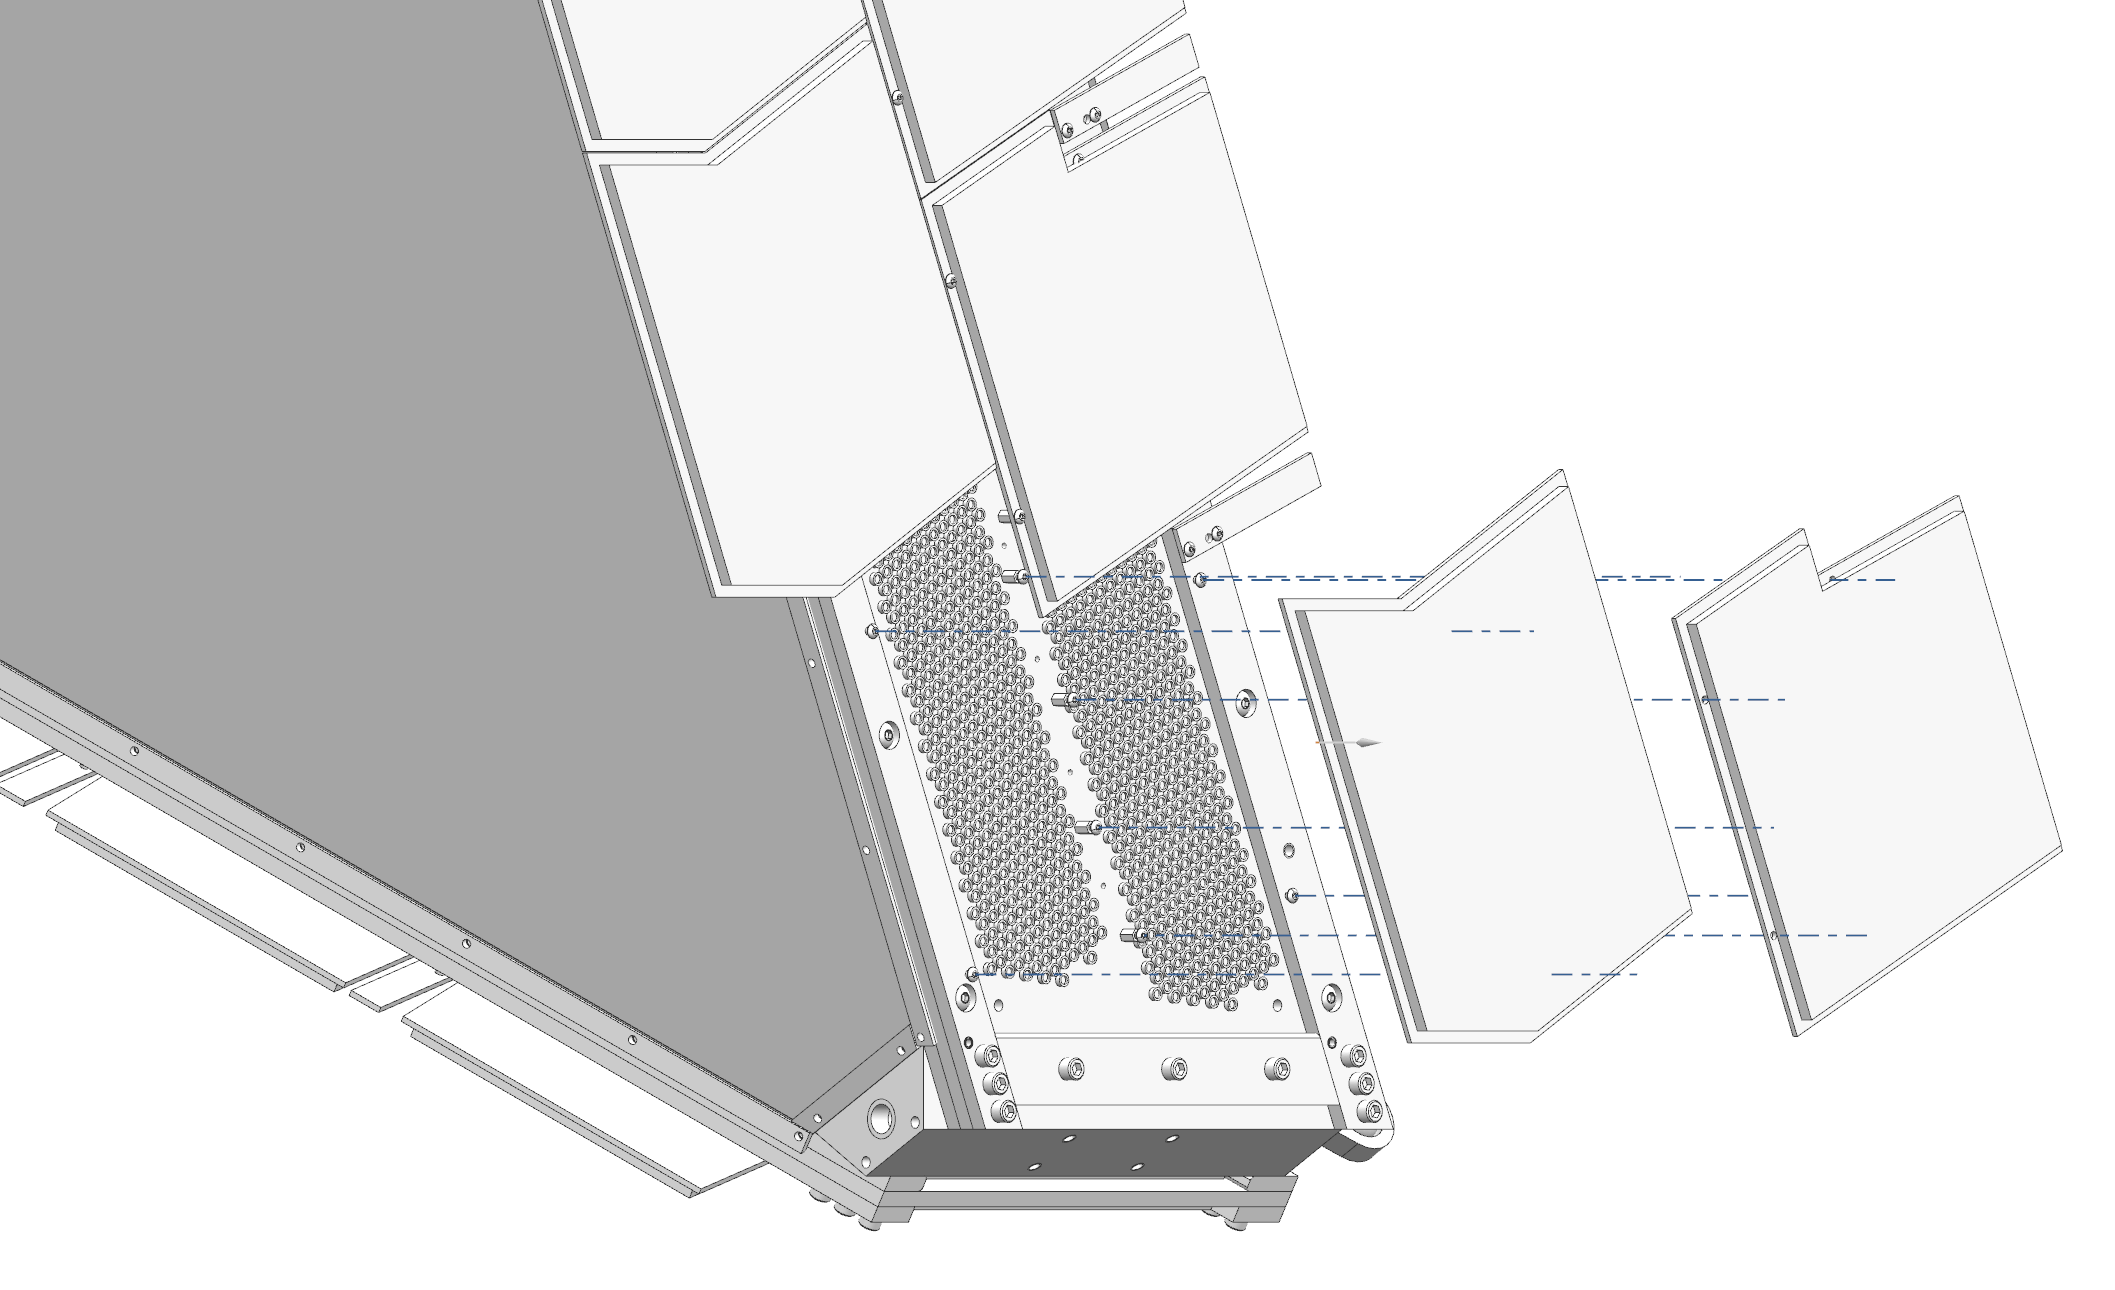
\includegraphics[width=0.18\textwidth,natwidth=610,natheight=642]{img/mounting-stb.png}}}
\end{picture}
\caption{\small{A sketch showing an on-chamber STB board being mounted.}}
\label{mounting-stb}
\end{figure}
%%%%%%%%%%%%%%%%%%%%%%%%%%%%%%%%%%%%%%%%%%%%%%%%%%%%%%%%%%%%%%

Now the chamber was ready for ``burn-in'' and ``pre-testing''.

\subsection{Burn-in and Pre-testing}

When drift chambers are first turned on, they typically draw fairly high
``dark'' currents, even at low voltages.  The standard procedure is to
slowly raise the high voltage, wait for a certain time period during
which the current subsides and raise the voltage again, and so on.
For our chambers, the typical time period was an hour and the typical
voltage step was 75~V.  For comparison, 100 - 120~V is approximately the 
``doubling voltage'' of
our chambers (the voltage step that increases the gain by a factor
of two).  The total time of ``burn-in'' for each chamber varied from one to three days.
Visual observation of good signals on an oscilloscope completed
the pre-testing.

\subsection{Installation and Survey}

The chambers are attached by ball-and-socket joints to rods that are attached
on the other end by ball-and-socket to the toroidal magnet frame.
After the initial installation, the chambers were moved to an approximate
working location.  Then, with the survey crew's information, the chamber location
was fine tuned by lengthening or shortening the rods with fine-pitch screw adjustments.
In this way the final chamber positioning was performed with sub-millimeter accuracies as
determined by the survey group's laser positioning system.

The installation of 18 chambers took months to accomplish and the survey crew's work
was hindered at times by obscured views of some of the fiducial marks on the 
chambers.  We checked and updated the survey information with a later 
``straight-track'' zero-field alignment run and analysis procedure (see Section~\ref{align}
for details of the alignment).
Although most of the alignment numbers were verified to sub-millimeter accuracy, there
were a few parameters that were off by as much as 2 mm.

Of particular note regarding the ``rod and ball-and-socket'' mounting scheme:
\begin{itemize}
\item by design, changing the length of any or all of the six links will
move the chamber in position and/or angle but will not apply stress to the
chamber;
\item once installed and surveyed, the chamber can be moved out to maintenance
position by changing only one of the link lengths;
\item this ``one link'' motion is reproducible to sub-millimeter accuracy, reducing the time
and manpower required for maintenance and repair.  In a matter of 8 hours, a chamber 
can be moved to ``maintenance position'', repaired, and moved back to installation
position without the need for a re-survey. Figure~\ref{maintenance-position} shows a single
chamber in its maintenance position.
\end{itemize}

%%%%%%%%%%%% Figure : chamber in maintenance position  %%%%%%%%%%%%%%%%%%%%%%%%%%%
\begin{figure}[htbp]
\vspace{4.3cm}
\begin{picture}(50,50)
\put(0,0)
{\hbox{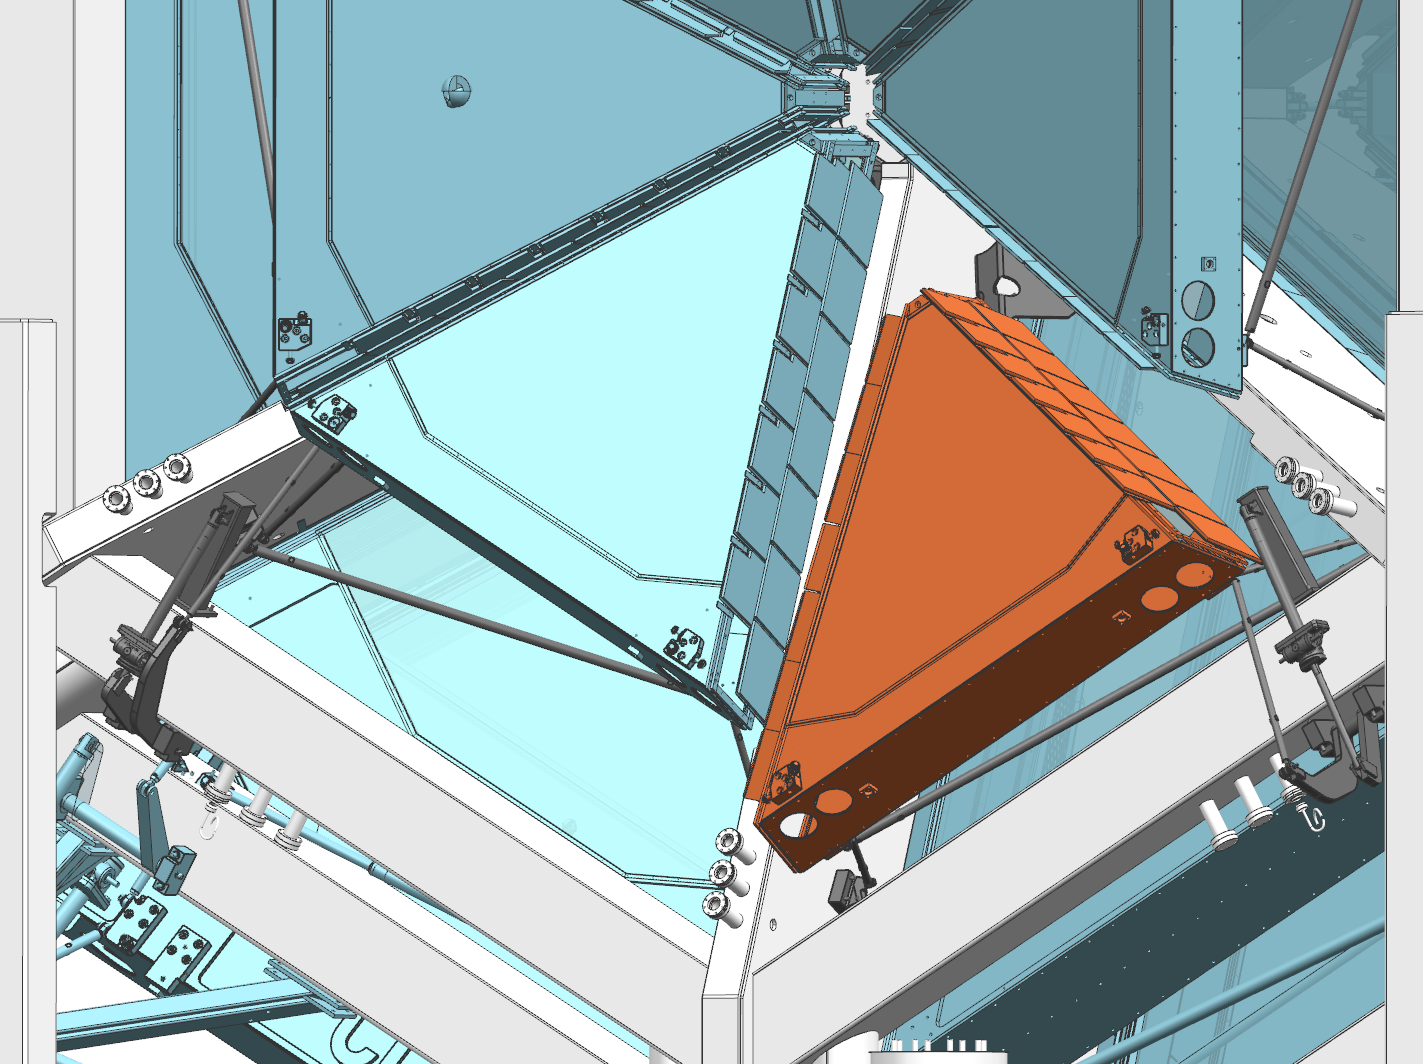
\includegraphics[width=0.28\textwidth,natwidth=610,natheight=642]{img/maintenance_04.png}}}
\end{picture}
\caption{\small{A view of the drift chambers mounted onto the torus magnet, with one R1
chamber moved out to its maintenance position.}}
\label{maintenance-position}
\end{figure}
%%%%%%%%%%%%%%%%%%%%%%%%%%%%%%%%%%%%%%%%%%%%%%%%%%%%%%%%%%%%%%%
